\documentclass[tikz,border=4pt]{standalone}
\usepackage{pgfplots}
\pgfplotsset{compat=1.16}
\pgfplotsset{
  bode/.style={
    width=6.4cm, height=4.4cm, xmin=0.01, xmax=100,
    grid=both, major grid style={gray!55}, minor grid style={gray!20},
    tick label style={font=\footnotesize}, label style={font=\small},
    title style={font=\small}, xlabel={$\omega/\omega_{p0}$ [rad/s]},
  },
  bode mag/.style={bode, ymin=-50, ymax=50, ytick={-40,-20,0,20,40},
    ylabel={$|G|_{\mathrm{dB}}$}, title={Modulo}},
  bode fase/.style={bode, ymin=-100, ymax=100, ytick={-90,-45,0,45,90},
    ylabel={$\varphi$ [$^\circ$]}, title={Fase}},
}
\begin{document}
% G(j w) = 1/(j w)
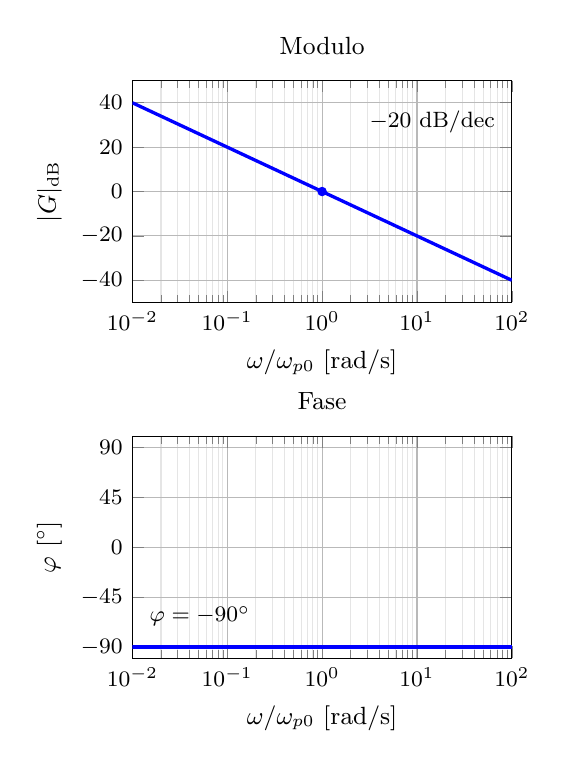
\begin{tikzpicture}
% ---------- modulo ----------
\begin{semilogxaxis}[bode mag, name=mag]
  \addplot[blue, very thick, domain=-2:2, samples=2] ({10^x}, {-20*x});
  \addplot[only marks, mark=*, mark size=1.5pt, blue] coordinates {(1,0)};
  \node[anchor=south west, font=\footnotesize] at (axis cs:2.5,22) {$-20$ dB/dec};
\end{semilogxaxis}
% ---------- fase ----------
\begin{semilogxaxis}[bode fase, at={(mag.south west)}, yshift=-1.7cm, anchor=north west]
  \addplot[blue, very thick] coordinates {(0.01,-90) (100,-90)};
  \node[anchor=south west, font=\footnotesize] at (axis cs:0.012,-80) {$\varphi=-90^\circ$};
\end{semilogxaxis}
\end{tikzpicture}
\end{document}